\documentclass[10pt,a4paper,fleqn]{article}
\usepackage[utf8]{inputenc}
\usepackage{amsmath}
\usepackage{amsfonts}
\usepackage{amssymb}
\usepackage{fullpage}
\usepackage{amsthm}
\usepackage{graphicx}

\newcommand{\example}[1]{\textbf{Example}: \emph{#1}}
\newcommand{\justification}[1]{\text{[\textbf{#1}]}}

\newcommand{\challenge}{(\emph{Challenge}) }
\newcommand{\dprime}{\prime\prime}

\author{James Camano}
\title{Mathematical Induction and Proofs by Induction}
\begin{document}
	\maketitle
	\newpage
	
	% Introduction	
	\part{Mathematical Induction}
		% Begin with a review of proofs
		We start our discussion with a quick review of proofs in mathematics.
		% Direct Proofs vs. Indirect Proofs
		\section{Direct vs. Indirect Proof Structure}
			In the words of one of my Computer Science professors, a proof is a convincing argument. \\ 
			Proof methods (i.e. the ways to argue a statement's validity or invalidity) can be separated into two groups: \emph{Direct} and \emph{Indirect} 	  methods. In other words, the way that a mathematician uses logic to prove some statement can be thought to be in one of these ``styles".
			
		\subsection{Direct Proofs}
			A proof which has a direct proof structure can be thought of as using known facts to prove a statement, without resorting to an alternative method. We provide an example. \\
			
		\noindent \example{Prove that the sum of two odd numbers is an even number.}
		\begin{proof}
			Let $a$ and $b$ be odd numbers. Then, we must have
			\begin{align*}
				&a = 2n + 1, \quad \text{ and}   \\
				&b = 2m + 1; \quad \text{for } n,m \in \mathbb{Z}
			\end{align*}			
			This is from the definition of odd numbers (note that number $n$ is even if $n = 2k, k \in \mathbb{Z}$.) Adding $a$ and $b$, we immediately retrieve the desired result:
			\begin{align*}
				a + b &= (2n + 1) + (2m + 1) \quad \justification{by definition of $a$ and $b$} \\
						 &= (2n + 2m) + (1 + 1) \quad \justification{by the commutative property of $\mathbb{Z}$} \\
						 &= 2(n+m) + 2				\quad \justification{factoring} \\
						 &= 2(n+m+1)				\quad \justification{factoring}
			\end{align*}		
			Since the sum of an integer and another integer will always be an integer, we conclude that $a+b$, by definition, is an even number, as wanted.
		\end{proof}
	One might regard the notion of a direct proof as so `trivial' that it is hard to understand. Perhaps contrasting a direct proof against an indirect proof may bring some clarity.
	
	\subsection{Indirect Proofs}
	% Indirect Proofs
	An indirect proof method is a method in which the proof does not explicitly prove the desired predicate \footnote{A \emph{predicate} is a formal statement in mathematics that can either be seen as a true statement or a false statement. Predicates are what this note might informally refer to as `statements'}. An indirect proof resorts to proving another statement, for whose validity it immediately follows (or in other words, implies) the desired predicate's validity. We provide a classic example. \footnote{This is known as Euclid's Argument of infinite primes.} \\
		
		% Euclid's Argument
		\noindent \example{Prove that there are infinitely many prime numbers.}
		\begin{proof} 
			Let $p$ be a prime number. Then $p$ satisfies the following conditions:
				\begin{enumerate}
					\item $p \in \mathbb{N}$
					\item $p \geq 2$, and
					\item The only factors of $p$ are $1$ and $p$, that is, no number other than $1$ and $p$ divides $p$ evenly.
				\end{enumerate}
			Suppose to the contrary that there exists a finite number $n$ of prime numbers. \\
			Then,we may, theoretically, gather the entire collection of these primes. Let this collection be described as $F = \{p_1, p_2, ..., p_n\}$ \footnote{This is known as a set, and the way we have described it is called an \emph{exhaustive} description of a set.}. \\
			Let the number $p \prime $ be the \emph{product of all of the primes in $F$}. We must have:
			\begin{align*}
				p' = p_1 \cdot p_2 \cdot ... \cdot p_n
			\end{align*}
			We see that $p'$ is definitely divisible by all of the primes in existence (in $F$, by supposition). \\
			Consider the number $p \dprime = p \prime + 1$. Notice that this number is not divisible by any of the primes in existence - to see this, notice that by dividing $p \dprime $ by any $p \in F$, we always will get a remainder of 1 \footnote{Rigorously, we would consult the division algorithm - however, I believe the preceding argument naturally suffices}. \\
			
			It becomes clear that the only factors of $p \dprime$ are 1, and $p \dprime$ itself. We have effectively generated a new prime number that was not in $F$. Suppose we added $p \dprime$ to $F$ to achieve a new collection $F \prime$. Then, by the same arguments detailed in this proof, we can continuously generate new primes without bound! Thus, we see that we could not have possibly have defined a finite set $F$ of prime numbers in the first place, because $F$ was already infinite to begin with. The desired conclusion follows.
					
		\end{proof}
	
	The `indirect' portion of this proof is in the supposition statement. We suppose that the statement we are trying to prove is false, and by flawless logical reduction from this supposition, we reach a contradiction. We then argue that the only flaw in our logic was the supposition itself, so therefore, the actual desired conclusion must be true. Thus, by resorting to proving another related statement, the desired statement is proven. (This specific indirect proof method is known as a \emph{Proof by Contradiction.})
	
	% a simple diagram of proof structure
	\begin{figure}[h]
		\centering
		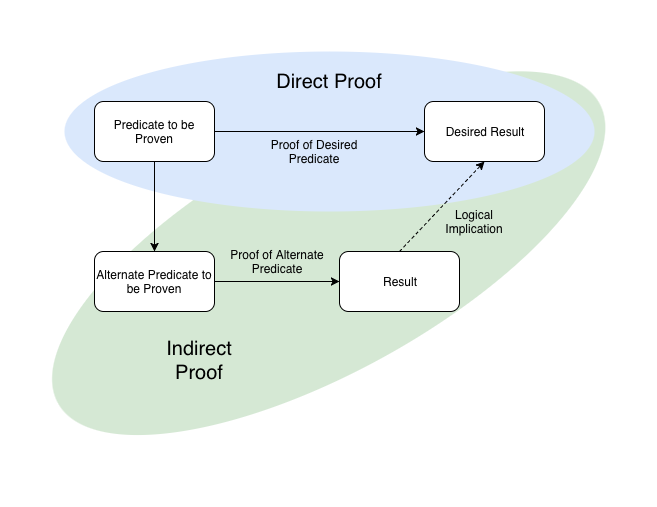
\includegraphics[scale=0.5]{res/direct_indirect.png}
		\caption{Depicting the algorithmic difference between the two types of proof structure.}
	\end{figure}
	
	\newpage
	
	\section{``Induction"?}
	
	\part{Questions}
		\begin{enumerate}
			\item Prove directly that the sum of an even integer and another even integer (not necessarily the same integer) is even.
			\subitem --- What can you conclude about the sum of an odd integer and an even integer? Can you directly prove it?
			\item \challenge Prove that any odd number is equal to a difference of squares \footnote{A difference of squares is of the form $(a^2 - b^2)$, where $a, b \in \mathbb{N}$}. 
			
			\item Prove $\sum_{i = 1}^{n} i^2 = \frac{n(n+1)(2n+1)}{6}$, by induction.
			\item Prove $\sum_{i = 1}^{n} i^3 = (\sum_{i = 1}^{n} i)^2 $.
			\item \challenge Prove by Induction that the degree-sum of the internal angles of $n$-sided polygon is equal to $(n-2)*180$
		\end{enumerate}
		
	
\end{document}